\section{/media/docs/progra/c++/compiladores1/proy2/godzilla/src/ Directory Reference}
\label{dir_000007}\index{/media/docs/progra/c++/compiladores1/proy2/godzilla/src/ Directory Reference@{/media/docs/progra/c++/compiladores1/proy2/godzilla/src/ Directory Reference}}


\begin{figure}[H]
\begin{center}
\leavevmode
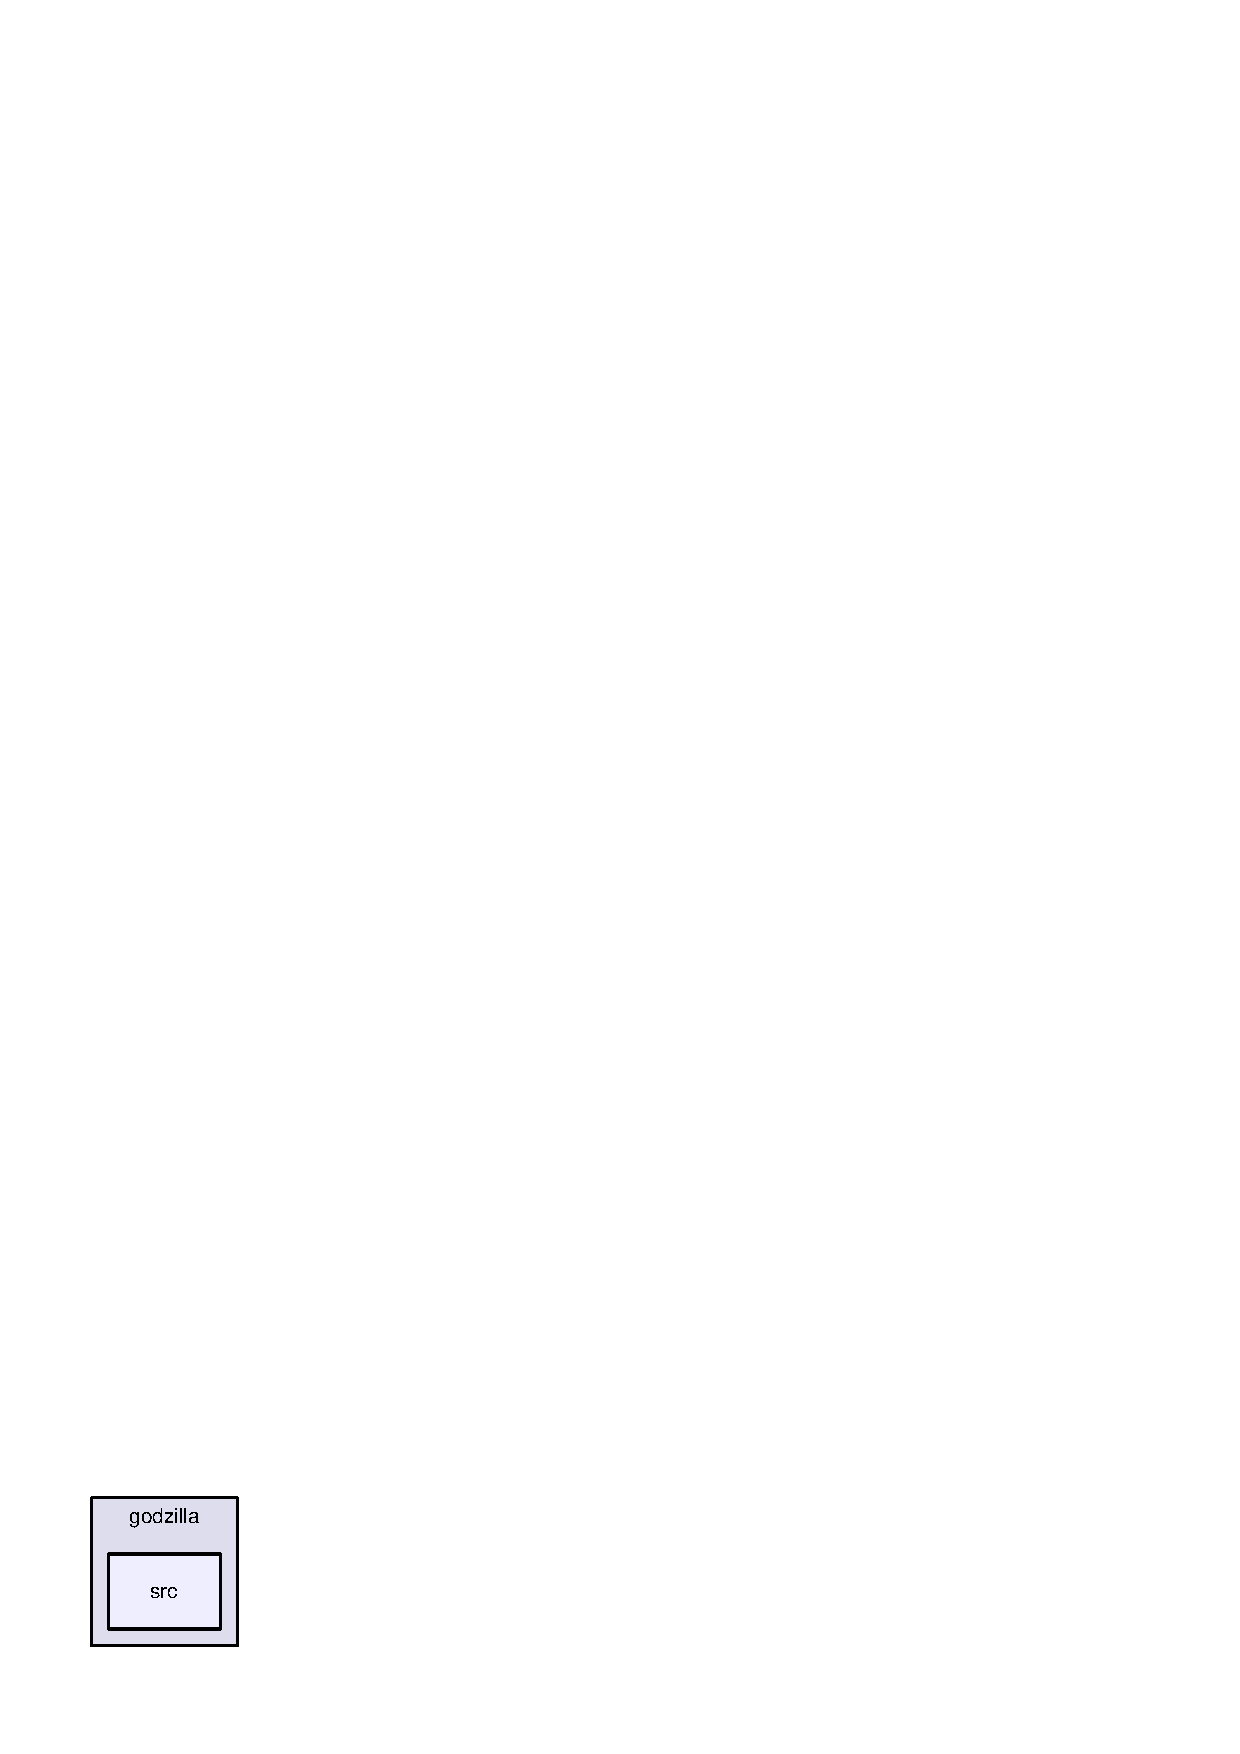
\includegraphics[width=61pt]{dir_000007_dep}
\end{center}
\end{figure}
\subsection*{Archivos}
\begin{CompactItemize}
\item 
archivo {\bf ast.c}
\begin{CompactList}\small\item\em Implementacion del arbol de sintaxis abstracta. \item\end{CompactList}

\item 
archivo {\bf ast.h}
\begin{CompactList}\small\item\em Definiciones y estructura del arbol de sintaxis abstracta. \item\end{CompactList}

\item 
archivo {\bf browser.cpp}
\begin{CompactList}\small\item\em Implementacion de la clase browser\-Dock. \item\end{CompactList}

\item 
archivo {\bf browser.h}
\begin{CompactList}\small\item\em Definiciones de la clase browser\-Dock. \item\end{CompactList}

\item 
archivo {\bf colaerr.c}
\begin{CompactList}\small\item\em Implementacion de la cola almacenadora de errores . \item\end{CompactList}

\item 
archivo {\bf colaerr.h}
\begin{CompactList}\small\item\em Definiciones de la cola almacenadora de errores . \item\end{CompactList}

\item 
archivo {\bf constantes.h}
\begin{CompactList}\small\item\em Constantes utilizadas por el arbol de sintaxis abstracta. \item\end{CompactList}

\item 
archivo {\bf godzilla.cpp}
\begin{CompactList}\small\item\em Implementacion de la Widged principal del GUI. \item\end{CompactList}

\item 
archivo {\bf godzilla.h}
\begin{CompactList}\small\item\em defiinicion de la Widged principal del GUI. \item\end{CompactList}

\item 
archivo {\bf main.cpp}
\begin{CompactList}\small\item\em Punto de entrada del programa. \item\end{CompactList}

\item 
archivo {\bf parserheader.h}
\begin{CompactList}\small\item\em interfaz entre el GUI y el parser. \item\end{CompactList}

\item 
archivo {\bf symtab.c}
\begin{CompactList}\small\item\em Implementacion de la tabla de simbolos.Incluye la implementacion de rutinas de insercion, busqueda y eliminacion. \item\end{CompactList}

\item 
archivo {\bf symtab.h}
\begin{CompactList}\small\item\em Estructuras de la tabla de simbolos.Incluyendo rutinas de insercion, busqueda y eliminacion. \item\end{CompactList}

\end{CompactItemize}
